\documentclass[ 12pt]{article}
%\setlength{\columnsep}{2cm}

%\usepackage{cite} 
\usepackage[round,authoryear,numbers]{natbib}
\usepackage[french]{babel}
\usepackage[utf8]{inputenc}
\usepackage{graphicx} %pour mettre des figures dans multicol avec l'environnement figure*

\usepackage[T1]{fontenc} % Use 8-bit encoding that has 256 glyphs
%\linespread{1.05} % Line spacing - Palatino needs more space between lines
%\usepackage{microtype} % Slightly tweak font spacing for aesthetics

\usepackage[hmarginratio=1:1,top=10mm]{geometry} % Document margins
\usepackage[textfont=it]{caption} % Custom captions under/above floats in tables or figures
\usepackage{booktabs} % Horizontal rules in tables
%\usepackage{float} % Required for tables and figures in the multi-column environment - they need to be placed in specific locations with the [H] (e.g. \begin{table}[H])
\usepackage{hyperref} % For hyperlinks in the PDF

\usepackage{bm}
\usepackage{amsfonts}
\usepackage{amsmath}
\usepackage{amssymb}
\usepackage{tabularx}

\usepackage{titlesec} % Allows customization of titles
\renewcommand\thesection{\Roman{section}} % Roman numerals for the sections
\renewcommand\thesubsection{\arabic{section}.\arabic{subsection}} % Roman numerals for subsections
\titleformat{\section}[block]{\bfseries\centering}{\thesection.}{1em}{}[{\titlerule[1.2pt]}] % Change the look of the section titles
\titleformat{\subsection}[block]{\bfseries}{\thesubsection.}{1em}{} % Change the look of the section titles
\renewcommand\thesubsubsection{\small{\arabic{section}.\arabic{subsection}.\arabic{subsubsection}}}
\titleformat{\subsubsection}[block]{\bfseries}{\thesubsubsection}{0.5em}{}
\titleformat*{\paragraph}{\vspace{-0.3cm}\small\bfseries}

\newcommand{\tbullet}{$\vcenter{\hbox{\tiny$\bullet$}}~$}

\usepackage{fancyhdr} % Headers and footers
\pagestyle{fancy} % All pages have headers and footers
\fancyhead{} % Blank out the default header
\fancyfoot{} % Blank out the default footer
\renewcommand{\headrulewidth}{0pt} %pour enlever la ligne du header
%\fancyhead[C]{titre, date, noms...	} % Custom header text
%\fancyfoot[RO,RE]{\thepage} % Custom footer text
%\fancyfoot[LO,LE]{A. DINSENMEYER, \today}
%\renewcommand{\footrulewidth}{0.4pt} 

%modif des espacement avant et après l'environnement equation
\let\oldequation=\equation
\let\endoldequation=\endequation
\renewenvironment{equation}{\vspace{-0.2cm}\begin{oldequation}}{\vspace{-0.2cm}\end{oldequation}}
 
%agrandissement de la zone de texte
%\addtolength{\oddsidemargin}{-1cm}
%\addtolength{\evensidemargin}{-1cm}
%\addtolength{\textwidth}{2cm}
%\addtolength{\topmargin}{-0.7cm}
\addtolength{\textheight}{1cm}

\usepackage{color}
\usepackage[color=blue!20]{todonotes}
\usepackage{mathtools}

%pour écrire du pseudo code :
\usepackage{algorithm}
\usepackage{algorithmic}

\usepackage{hyperref}
\hypersetup{
     colorlinks   = true,
     citecolor    = blue!90
}

\newcommand{\dd}{\partial}
\newcommand{\ok}{ \textcolor{orange}{\bfseries \textsc ok }}
\newcommand{\diag}[1]{\lceil#1\rfloor}
\newcommand{\e}{\mathrm{e}}
\newcommand{\tr}[1]{\operatorname{Trace}\!\left(#1\right)}


\usepackage{subcaption}
\usepackage{tabulary}
\usepackage{pgfplots} 

\graphicspath{{/home/adinsenmey/Bureau/these_2017/MCMC_Samplers/img/}}

\everymath{\displaystyle}
%----------------------------------------------------------------------------------------
%	TITLE SECTION
%----------------------------------------------------------------------------------------

\title{\vspace{-12mm}\fontsize{14pt}{14pt}\selectfont\textbf{Analyse Factorielle parcimonieuse avec priors Bernoulli-Gaussiens sur les facteurs}} % Article title
%\author{
%\large{Alice \textsc{Dinsenmeyer}}\\[2mm] % Your name %\thanks{}
%\normalsize University of California \\ % Your institution
%\normalsize \href{mailto:john@smith.com}{john@smith.com} % Your email address
%\vspace{-5mm}
%}
\date{\vspace{-1cm}Décembre 2018
}

%----------------------------------------------------------------------------------------

\begin{document}
\maketitle


\section{Modèle 1 : Parcimonie par priors exponentiels}
L'objectif est d'améliorer le modèle suivant : 
\begin{equation}
        \bm{y}_i= \bm{L  \diag{q} c }_i + \bm{n}_i
\end{equation}
\begin{center}
\begin{tabular}{l | l l}
\hline \textbf{Priors} & \textbf{Hyperpriors} \\ \hline 

$ \bm{L} \sim \mathcal{N}_c (0,\frac{\bm{I}_{MK}}{K})$ & \\[1em]
$\bm{c} \sim \mathcal{N}_c (0, \bm{\diag{\gamma^2}})$ & $\bm{\gamma^2} \sim \mathcal{IG}(a_{\gamma},b_{\gamma})$\\[1em]	
\fbox{ $\bm{q} \sim\mathcal{E}xp(\bm{a}_q)$} & \\[1em]	
$\bm{n}| \beta^2 \sim \mathcal{N}_c (0, \beta^2 \bm{\diag{\sigma^2}}) $ & $\bm{\sigma^2} \sim \mathcal{IG}(a_{\sigma},b_{\sigma})$&\\
														& $\beta^2 \sim \mathcal{IG}(a_{\beta},b_{\beta})$												
\end{tabular}
\end{center}
Ce modèle pose les problèmes résumés dans le tableau ci-dessous : 
\begin{center}
\renewcommand{\arraystretch}{1.8}
\begin{tabular}{m{0.45\textwidth} | m{0.45\textwidth}}
	\hline \textbf{Faiblesses rencontrées dans le modèle 1} & \textbf{Solutions proposées par le modèle 2}\\\hline\hline
	 $\bm{q}$ n'est pas normalisé, on ne peut donc pas observer la stabilité de la chaîne & $\bm{q}$ vaut 0 ou 1 ; toute la variance est portée par $\bm{c}$\\\hline
	 $\bm{q}$ et $\bm{c}$  risquent d'être fortement corrélés, ce qui peut nuire à la mélangeance des chaînes & Marginalisation partielle de l'échantillonneur\\\hline
	 Sensibilité des résultats au choix des hyperparamètres $\bm{a}_q$ & Échantillonnage de l'hyperparamètre dans une loi Bêta.
\end{tabular}
\end{center}




\section{Bibliographie}
Le chapitre 4 de la thèse de Charly Faure y est dédié, avec le modèle suivant : 
\begin{equation}
        \bm{y}= \bm{Hf}+ \bm{n}
\end{equation}
où $\bm{f} \sim \prod_i \mathcal{B}ern\mathcal{G}auss(f_i~;~ l,\gamma^2)$. L'échantillon $f_i$ est donc tiré soit dans une Gaussienne, soit dans un Dirac en 0 (cas particulier d'une Gaussienne de variance nulle). Ce qui peut s'écrire : 
\begin{equation}
        \mathcal{B}ern\mathcal{G}auss(l,\gamma^2) = (1-l)\mathcal{N}_c(0,0) + l \mathcal{N}_c(0,\gamma^2)
\end{equation}

\cite{Ge2011} ont une approche similaire, en notant $\bm{f} \sim \mathcal{N}_c(0,\diag{\bm{q}}\gamma^2)$, où les éléments de $\bm{q}$ suivent une loi de Bernoulli.


\section{Calculs}
\subsection{Nomenclature}
\begin{tabular}{c c}
M & Nombre de micros\\
K & Nombre de facteurs\\
$I_{s}$ & Nombre de moyennes pour le calculs des CSM\\
$i$ & indice associé à une moyenne\\
$L_q$ & nombre d'éléments non-nuls du vecteur $\bm{q}$

\end{tabular}

\subsection{Modèle 2 : Parcimonie par priors bernoulliens}
On choisit un modèle hiérarchique avec la matrice de mixage $\bm{L}$, les facteurs $\bm{c}$ et les binaires $\bm{q}$ au même étage :
\begin{equation}
        \bm{y}_i= \bm{L  \diag{q} c }_i + \bm{n}_i
\end{equation}

\begin{center}
\begin{tabular}{l | l l}
\textbf{Priors} & \textbf{Hyperpriors} \\ \hline 

$ \bm{L} \sim \mathcal{N}_c (0,\frac{\bm{I}_{MK}}{K})$ & \\[1em]
$\bm{c} \sim \mathcal{N}_c (0, \bm{\diag{\gamma^2}})$ & $\bm{\gamma^2} \sim \mathcal{IG}(a_{\gamma},b_{\gamma})$\\[1em]	
 \fbox{$\bm{q} \sim \mathcal{B}ern(l)$} &  \fbox{$ l \sim \mathcal{B}eta(a_l,b_l)$}\\[1em]	
$\bm{n}| \beta^2 \sim \mathcal{N}_c (0, \beta^2 \bm{\diag{\sigma^2}}) $ & $\bm{\sigma^2} \sim \mathcal{IG}(a_{\sigma},b_{\sigma})$&\\
														& $\beta^2 \sim \mathcal{IG}(a_{\beta},b_{\beta})$ 														
\end{tabular}
\end{center} 
On note par la suite $\bm{\Omega}_n = \beta^2 \bm{\diag{\sigma^2}}$. Le paramètre $\beta$ est introduit par anticipation d'un modèle adapté au cas multirégime d'Airbus.

%\bigskip
%
%D'où les probabilités conditionnelles suivantes : 
%\begin{equation*}
%        \left[ \bm{y}_i | \infty_{-\bm{y}_i} \right] \propto \frac{\e^{- (\bm{y}_i-\bm{Lqc}_i)^H \bm{\Omega}_n^{-1}(\bm{y}_i - \bm{Lqc}_i) }}{|\bm{\Omega}_n|}
%\end{equation*}





\subsection{Posteriors}

% l
\subsubsection{Échantillonnage du paramètre de parcimonie $l$}
\begin{align*}
	\left[ l | \bm{q} \right] &\propto \mathcal{B}eta(l ; a_l,b_l) \prod_k^K  \mathcal{B}ern(q_k ; l)\\	
	&\propto \frac{\Gamma(a_l+b_l)}{\Gamma(a_l)\Gamma(b_l)} l^{a_l-1}(1-l)^{b_l-1} \prod_k^K l^{q_k}(1-l)^{1-q_k}\\
	& \propto \frac{\Gamma(a_l+b_l)}{\Gamma(a_l) \Gamma(b_l)}~ l^{a_l-1}~(1-l)^{b_l-1} ~ l^{\sum_k q_k}~(1-l)^{\sum_k 1-q_k}\\
	&\boxed{ \propto  \mathcal{B}eta( a_l + L_q  ,   b_l + K - L_q)}
\end{align*}

% Sc
\subsubsection{Échantillonnage en bloc de c}
\begin{align*}
	\left[ \bm{c}_i | \infty_{-\bm{c_i}} \right] &\propto   \left[ \bm{y}_i | \infty_{-\bm{y}_i} \right] \mathcal{N}_c (\bm{c}_i ; 0, \bm{q\gamma}^2)\\
	& \propto \frac{\e^{- (\bm{y}_i-\bm{Lqc}_i)^H \bm{\Omega}_n^{-1}(\bm{y}_i - \bm{Lqc}_i) }}{|\bm{\Omega}_n|}  \e^{\bm{c}_i^H \bm{\gamma}^{-2}\bm{c}_i}\\[1ex]
	& \propto \e^{ - (\bm{c}_i- \bm{\mu}_i)^H \bm{\Omega}^{-1}_{\bm{c}_i}     (\bm{c}_i- \bm{\mu}_i)  }	
\end{align*}
Par identification, on a : 
\begin{align*}
       \bullet \quad &\bm{c}_i^H \bm{\Omega}^{-1}_{\bm{c}_i} \bm{c}_i =   \bm{c}_i^H \left( \bm{qL}^H \bm{\Omega}_n^{-1} \bm{Lq}+ \bm{\gamma}^{-2} \right) \bm{c}_i\\~\\
        \bullet\quad & \bm{\Omega}^{-1}_{\bm{c}_i} \bm{\mu}_i = \bm{q}^H\bm{L}^H \bm{\Omega}_n^{-1} \bm{y}_i
\end{align*}
Finalement : \\

\begin{center}
	\fbox{ \parbox{0.6\linewidth}{
		\begin{equation}
			\left[ \bm{c}_i | \infty_{-\bm{c_i}} \right]  \propto \mathcal{N}_c (\bm{\mu}_i, \bm{\Omega}_{\bm{c}_i})
			\label{eq:c}
		\end{equation}
		\begin{align*}
			&\text{où : } \quad \bm{\Omega}_{\bm{c}_i} = \left( \bm{qL}^H\bm{\Omega}_n^{-1} \bm{Lq}+ \bm{\gamma}^{-2} \right)^{-1} \\
			& \text{et} \quad
			\bm{\mu}_i = \bm{\Omega}_{\bm{c}_i}  \bm{q}^H\bm{L}^H\bm{\Omega}_n^{-1} \bm{y}_i
		\end{align*}
		}}
\end{center}


Dans le cas où le nombre de moyenne est suffisamment grand, on peut échantillonner directement la matrice interspectrale \hbox{$\bm{S_{cc}} =  \mathbb{E}\{\bm{c}_i\bm{c}_i^H\}$}. On a : 
\begin{equation*}
	    \bm{c}_i = \bm{\mu}_i + \bm{x}_i \quad\text{avec}\quad \bm{x}_i \sim \mathcal{N}_c(0, \bm{\Omega}_{\bm{c}_i}),
\end{equation*}
donc : 
\begin{equation*}
        \mathbb{E}\{\bm{c}_i\bm{c}_i^H\} =  \mathbb{E}\{\bm{\mu}_i \bm{\mu}_i^H\} + \mathbb{E}\{\bm{x}_i \bm{x}_i^H\} + \underbrace{ 2\mathbb{E}\{\bm{x}_i \bm{\mu}_i^H\}}_{\rightarrow 0 \text{ quand } I_{s}\rightarrow \infty},
\end{equation*}
avec : 
\begin{align*}
& \bullet \quad\mathbb{E}\{\bm{x}_i \bm{x}_i^H\} = \bm{W}_c \sim \mathcal{W}(\bm{\Omega}_{\bm{c}_i} , I_{s})\\
& \bullet \quad  \mathbb{E}\{\bm{\mu}_i \bm{\mu}_i^H\}  =  \bm{\Omega}_{\bm{c}_i} \bm{q}^H\bm{L}^H  \bm{\Omega}_n^{-1}\bm{S}_{yy} \bm{Lq}  \bm{\Omega}_{\bm{c}_i}^H
\end{align*}

 

% L
\subsubsection[]{Échantillonnage de $\bm{L}$}
La matrice $\bm{L}$ est vectorisée de manière à écrire une matrice de covariance pour la postérieure qui soit à 2 dimensions. On note $\bm{\lambda}=\operatorname{vec}(\bm{L})$
\begin{align*}
	\left[ \bm{\lambda}| \infty_{-\bm{\lambda}}  \right] \propto \prod_i^{I_{s}} [\bm{y}_i | \infty_{-\bm{y}_i}][\bm{\lambda}]
\end{align*}
Or : 
\begin{equation}
        \operatorname{vec}(\bm{y}_i) = \bm{y}_i = \operatorname{vec}(\bm{Lqc}_i ) + \bm{n}_i  = \left( \bm{c}_i^T \bm{q} \otimes \bm{I}_M \right) \bm{\lambda} + \bm{n}_i,
\end{equation}
donc : 
\begin{align*}
        \left[ \bm{\lambda}| \infty_{-\bm{\lambda}}  \right] &\propto \e^{-\sum_i  \left( \bm{y}_i -  \left( \bm{c}_i^T \bm{q} \otimes \bm{I}_K \right) \bm{\lambda} \right) ^H \bm{\Omega}_n^{-1}  \left( \bm{y}_i -  \left( \bm{c}_i^T \bm{q} \otimes \bm{I}_M \right) \bm{\lambda} \right) }
        \e^{- \bm{\lambda}^H K\bm{I}_{MK} \bm{\lambda} }\\
&\propto \e^{ - (\bm{\lambda}- \bm{\mu}_\lambda)^H \bm{\Omega}^{-1}_{\bm{\lambda}}     (\bm{\lambda}- \bm{\mu}_\lambda)  }
\end{align*}
Comme précédemment, par identification, on a finalement : \\

\begin{center}
	\fbox{ \parbox{0.6\linewidth}{
		\begin{equation}
		 	 \left[ \bm{\lambda}| \infty_{\bm{\lambda}}  \right] \propto  \mathcal{N}_c( \bm{\mu}_\lambda , \bm{\Omega}_{\bm{\lambda}})
		\end{equation}
		\begin{align*}
			\text{où : } \quad \bm{\Omega_\lambda} &= \left(  \sum_i (\bm{c}_i^T \bm{q} \otimes \bm{I}_{M} )^H \bm{\Omega}_n^{-1} (\bm{c}_i^T \bm{q} \otimes \bm{I}_{M} )    + K\bm{I}_{MK}  \right)^{-1}\\
			&=\left( (\bm{q}\bm{S}_{cc}^* \bm{q}) \otimes (\bm{\Omega}_n^{-1}) + K\bm{I}_{MK}   \right)^{-1}\\
			 \text{et} \quad \bm{\mu}_\lambda & = \bm{\Omega_\lambda} \sum_i  (\bm{c}_i^T\bm{q} \otimes \bm{I}_M)^H \bm{\Omega}_n^{-1} \bm{y}_i\\
		 	&= \bm{\Omega_\lambda} \operatorname{vec}(\bm{\Omega}_n^{-1} \bm{S}_{yy}  \bm{\Omega}_n^{-1} \bm{Lq} \bm{\Omega_{\bm{c}_i} q} )
		\end{align*}
	}}
\end{center}

\textit{Notes : } - Ce dernier résultats s'obtient en remplaçant $\bm{c}_i$ par $\bm{\mu}_i$.\\
\indent - Les propriétés du produit de Kronecker sont les suivantes : 
\begin{align*}
\operatorname{vec}(ABC)&=(C^T \otimes A)\operatorname{vec}(B)\\
(A \otimes B)^T &= A^T \otimes B^T\\
(A \otimes B)^* &= A^* \otimes B^*\\
(A \otimes B)(C\otimes D)&=(AC)\otimes(BD)
\end{align*}
si les dimensions des matrices $A$, $B$, $C$ et $D$ le permettent.



% gamma
\subsubsection[]{Échantillonnage de $\bm{\gamma}^2$}

\paragraph{Cas où $\bm{\gamma}^2 = \gamma^2 \bm{I}_K$}
\begin{align*}
	\left[ \gamma^2| \bm{S}_{cc} \right] &\propto \prod_i [\bm{c}_i | \gamma^2] [\gamma^2]\\
	& \propto \frac{\e^{- \gamma^{-2} \sum_i \bm{c}_i^H \bm{c_i}}}{\gamma^{2I_{s}K}} \frac{\e^{- \gamma^{-2}b_\gamma}}{\gamma^{2(a_\gamma-1)}}	
\end{align*}

\begin{equation}
	\boxed{
       \left[ \gamma^2| \bm{S}_{cc} \right] \propto \mathcal{IG} \left( a_\gamma + K I_{s} , b_\gamma + \tr{\bm{S}_{cc}} \right)
       }
\end{equation}

%\textit{Discussion : } Pour  le paramètre de forme, vaut-il mieux prendre $a_\gamma + L_q I_{s}$, c'est à dire considérer uniquement la variance sur les facteurs non-nuls ? À noter que la $ \operatorname{Trace}(\bm{S}_{cc})$ ne somme n'implique que les éléments non-nuls.
\paragraph{Cas où $\bm{\gamma}^2 = \diag{\bm{\gamma^2 }} = \operatorname{diag}(\gamma^2_1, \dots, \gamma^2_k, \dots, \gamma_K^2)$}
\begin{align*}
	\left[ \gamma_k^2| \bm{S}_{cc} \right] \propto  \prod_i [\bm{c}_{ik} | \gamma_k^2] [\gamma^2_k]
\end{align*}
\begin{equation}
	\boxed{
       \left[ \gamma_k^2| \bm{S}_{cc} \right] \propto \mathcal{IG} \left( a_\gamma +  I_{s} , b_\gamma +\bm{S}_{cc_{kk}} \right)
       }
\end{equation}




% Sig
\subsubsection[]{Échantillonnage de $\bm{\sigma}^2$}
On considère un bruit hétéroskédastique : $\bm{\sigma}^2 = \operatorname{diag}(\sigma^2_1,\dots,\sigma^2_m,\dots,\sigma^2_M)$.
\begin{align*}
	\left[  \bm{\sigma}^2|\infty_{-\bm{\sigma}^2}\right] &\propto \prod_i [\bm{y_i}| \infty_{-\bm{y}_i}][\bm{\sigma}]\\
	&\propto  \frac{\e^{-\sum_i (\bm{y}_{i}-\bm{L} \bm{qc}_i)^H \beta^{-2}\bm{\sigma}^{-2} (\bm{y}_{i} - \bm{L} \bm{qc}_i) }}{\beta^2| \bm{\sigma}|^{I_s}} \frac{\e^{-\bm{\sigma}^{-2} b_\sigma}}{\bm{\sigma}^{2(a_\sigma-1)}}\\
	& \propto \frac{ \e^{-\tr{\beta^{-2} \bm{\sigma}^{-2} \overbrace{\sum_i \left\{   \bm{y}_i\bm{y}_i^H   
	+ \bm{Lqc}_i \bm{c}_i^H\bm{qL}^H
	-  \bm{y}_i\bm{c}_i^H \bm{qL}^H
	- \bm{Lqc}_i\bm{y}_i^H
	 \right\} }^{\bm{T}}} } }{|\bm{ \sigma}^2|^{I_s}}  \frac{\e^{-\bm{\sigma}^{-2} b_\sigma}}{\bm{\sigma}^{2(a_\sigma-1)}}
\end{align*}
On réinjecte $\bm{c}_i = \bm{\mu}_i + \bm{x}_i $ et on suppose que $\mathbb{E}(\bm{x}_i\bm{y}_i^H)\approx0$. En notant :
\begin{equation*}
        \bm{P}=\bm{Lq \Omega}_{c_i} \bm{qL}^H \bm{\Omega}_n^{-1} = \bm{P}^H,
\end{equation*}
on  a : $\displaystyle \bm{Lq\mu}_i = \bm{Py}_i$. Finalement : 
\begin{align*}
	\bm{T} &= \bm{S}_{yy} + \bm{LqW}_c \bm{qL}^H + \bm{PS}_{yy}\bm{P}
	- \bm{S}_{yy}\bm{P}
	- \bm{PS}_{yy}\\
	& = (\bm{I}_M -\bm{P}) \bm{S}_{yy} (\bm{I}_M -\bm{P}) + \bm{LqW}_c \bm{qL}^H
\end{align*}	

\begin{equation}
	\boxed{
	\left[	\sigma_m^2 |\infty_{-\sigma_m^2} \right] \propto  \mathcal{IG} \left( a_\sigma + MI_s , b_\sigma + \beta^{-2} \bm{T}_{mm}\right)
	}
\end{equation}


%beta 
\subsubsection[]{Échantillonnage de $\beta^2$}
De manière similaire à l'échantillonnage de $\sigma_m$ : 
\begin{align*}
	\left[ \beta^2 | \infty_{-\beta^2} \right] &\propto  \prod_i [\bm{y_i}| \infty_{-\bm{y}_i}][\beta^2]\\
	& \propto \frac{\e^{-\beta^{-2}\tr{\bm{\sigma^{-2}\bm{T}}}}}{|\beta^{2}\bm{I}_M|^{I_s}} \frac{\e^{-\beta^{-2}b_\beta}}{\beta^{2(a_\beta-1)}}
\end{align*}


\begin{equation}
	\boxed{
	\left[	\beta^2 |\infty_{-\beta^2} \right] \propto  \mathcal{IG} \left( a_\beta + MI_s , b_\beta + \tr{\bm{\sigma^{-2}\bm{T}}}\right)
	}
\end{equation}

% q
\subsubsection[]{Échantillonnage des binaires du vecteur $\bm{q}$}

\paragraph{Sans marginalisation}
\begin{align*}
	\left[q_k | \infty	_{-q_k}  \right] &\propto \prod_i  \left[ \bm{y}_i |q_k, \infty_{-\bm{y}_i} \right] [q_k]\\
	&\propto  \frac{\e^{-\sum_i (\bm{y}_i-\bm{Lqc}_i)^H \bm{\Omega}_n^{-1}(\bm{y}_i - \bm{Lqc}_i) }}{|\bm{\Omega}_n|^{I_s}}   l^{q_k}(1-l)^{1-q_k}\\
	& \propto \e^{-\tr{  \bm{\Omega}_n^{-1}  \bm{T}(q_k) } -q_k \ln\left( \frac{1}{l}-1 \right)}\\
	& \propto \e^{- g(q_k)}
\end{align*}
Le changement d'état d'un binaire se traduit par l'ajout de la quantité $\delta_k = (-1)^{q_k}$. On note $q_{k_{mod}}=q_k + \delta_k$.
La probabilité que le binaire change d'état est : 
\begin{align*}
	\left[q_{k_{mod}} | \infty	_{-q_k}  \right] & \propto  \prod_i  \left[ \bm{y}_i | q_{k_{mod}}, \infty_{-\bm{y}_i,\bm{c}} \right][q_{k_{mod}}]\\
	& \propto \e^{-\tr{  \bm{\Omega}_n^{-1}  \bm{T}(q_{k_{mod}}) }  -q_{k_{mod}} \ln\left( \frac{1}{l}-1 \right)}\\
	& \propto \e^{- g(q_{k_{mod}})}
\end{align*}

Pour que la somme de ces deux probabilité soit égale à 1, il faut les normaliser. La probabilité qu'un binaire change d'état est alors : 
\begin{align*}
	\left[q_{k_{mod}} | \infty_{-q_k}  \right] & =  \frac{ \e^{- g(q_{k_{mod}})}}{ \e^{- g(q_{k_{mod}})} +\e^{- g(q_{k})}}  \\[1ex]
	&\boxed{= \frac{1}{1 + \e^{- \left(g(q_{k}) -   g(q_{k_{mod}})\right)}}}
\end{align*}
Un échantillon $t \sim \mathcal{U}(0,1)$ est comparé à $\left[q_{k_{mod}} | \infty_{-q_k}  \right]$. S'il y est inférieur, le binaire change d'état, sinon il conserve son état actuel.\\
En pratique, comme $\bm{T}$ peut prendre de grandes valeurs (not. si $I_s$ est grand), le changement est accepté si $$-\ln\left(\frac{1}{t}-1\right) < g(q_{k}) -   g(q_{k_{mod}})$$


\paragraph{Avec marginalisation sur les facteurs $\bm{c}$}

\begin{align*}
	\left[q_k | \infty	_{-q_k,-\bm{c}}  \right] &\propto \prod_i  \left[ \bm{y}_i |q_k, \infty_{-\bm{y}_i,-\bm{c}} \right] [q_k]\\
\end{align*}
Or, 
\begin{equation}
        \left[ \bm{y}_i |q_k, \infty_{-\bm{y}_i,-\bm{c}} \right] = \mathcal{N}_c(0 , \underbrace{ \bm{Lq \gamma}^2 \bm{qL}^H + \bm{\Omega}_n}_{\bm{B}})
\end{equation}
Ce résultat est démontré en annexe~\ref{demo_marg}.

La posterior marginalisée sur le binaire $q_k$ est donc : 
\begin{align*}
	\left[q_k | \infty	_{-q_k,-\bm{c}}  \right] &\propto \frac{\e^{ - \sum_i  \bm{y}_i^H \bm{B}(q_k)^{-1}\bm{y}_i  }}{|\bm{B}(q_k)|^{I_s}}  l^{q_k}(1-l)^{1-q_k}\\
	& \propto \e^{-\tr{ \bm{B}(q_k)^{-1}\bm{S}_{yy}} - I_s\ln|\bm{B}(q_k)| - q_k \ln\left( \frac{1}{l}-1 \right)}\\
	& \propto \e^{- g(q_k)}
\end{align*}
De la même manière, la probabilité que le binaire change d'état est : 
\begin{align*}
	\left[q_{k_{mod}} | \infty	_{-q_{k_{mod}} ,-\bm{c}}  \right] & \propto  \frac{\e^{ - \sum_i  \bm{y}_i^H \bm{B}(q_{k_{mod}})^{-1}\bm{y}_i  }}{|\bm{B}(q_{k_{mod}})|^{I_s}}  l^{q_{k_{mod}}}(1-l)^{1-q_{k_{mod}}}\\
	 & \propto \e^{- g(q_{k_{mod}})}
\end{align*}
Après normalisation, le changement d'état du binaire est accepté si $$-\ln\left(\frac{1}{t}-1\right) < g(q_{k}) -   g(q_{k_{mod}})$$.



\section{Résultats et analyse}
\subsection{Paramètres de la simulation}

\begin{itemize}
        \item $M=20$
        \item $I_s = 10^4$
        \item SNR = 0 dB et -10 dB
        \item Nombre de fonction de base : 5
        \item Nombre de facteurs recherché : $K_r= M-1$  
        %\item Trace($\bm{S}_{pp}$)/M = 2.4     
\end{itemize}
Le paramètre $\beta^2$ est fixé à 1.

\paragraph{Priors}
\begin{itemize}
        \item $a_\sigma = b_\sigma = a_\gamma = b_\gamma = 0.01$ (paramètres pour un prior Gamma non-informatif)
        \item $a_l = b_l = 1$ (paramètre pour un prior bêta non-informatif)
\end{itemize}
\textit{Remarque : }Le choix d'un prior non informatif pour $\gamma^2$ est important pour la robustesse du solveur. De cette façon, si le nombre de binaires q est surestimé, une compensation pourra avoir lieu par une mise à 0 de certaines valeurs de $\gamma^2_k$ et du $\bm{c}_k$ correspondant.

\paragraph{Initialisation}
\begin{itemize}
        \item $\bm{L}_{(0)} \sim \mathcal{N}_c(0,\bm{I}/K_r)$
	\item $\sigma_{m(0)}^2=\tr{\bm{S}_{yy}}/M$
        \item  $\gamma_{k(0)}^2=0.3 \times \sigma_{m(0)}^2$ (hypothèse d'un SNR à -5 dB ($10\log_{10}(0.3)$)
        \item $q_{k(0)}=1$ 
\end{itemize}

\todo[inline]{
- avec marg/sans marg pour 4 initialisations\\
-comp avec modele 1\\
-comp q=1\\
-effet facteur d'échelle\\
-effet prior sur le param de parcimonie\\
-effet $\gamma^2_k$ sur modele 1(et prior non informatif)
}

\subsection{Comparaison du modèle 2 AVEC et SANS marginalisation}
On compare ici le cas où $\bm{q}$ est tiré (toujours en bloc) suivant une postérior marginalisée ou non.

\begin{figure}[H]
	\centering
	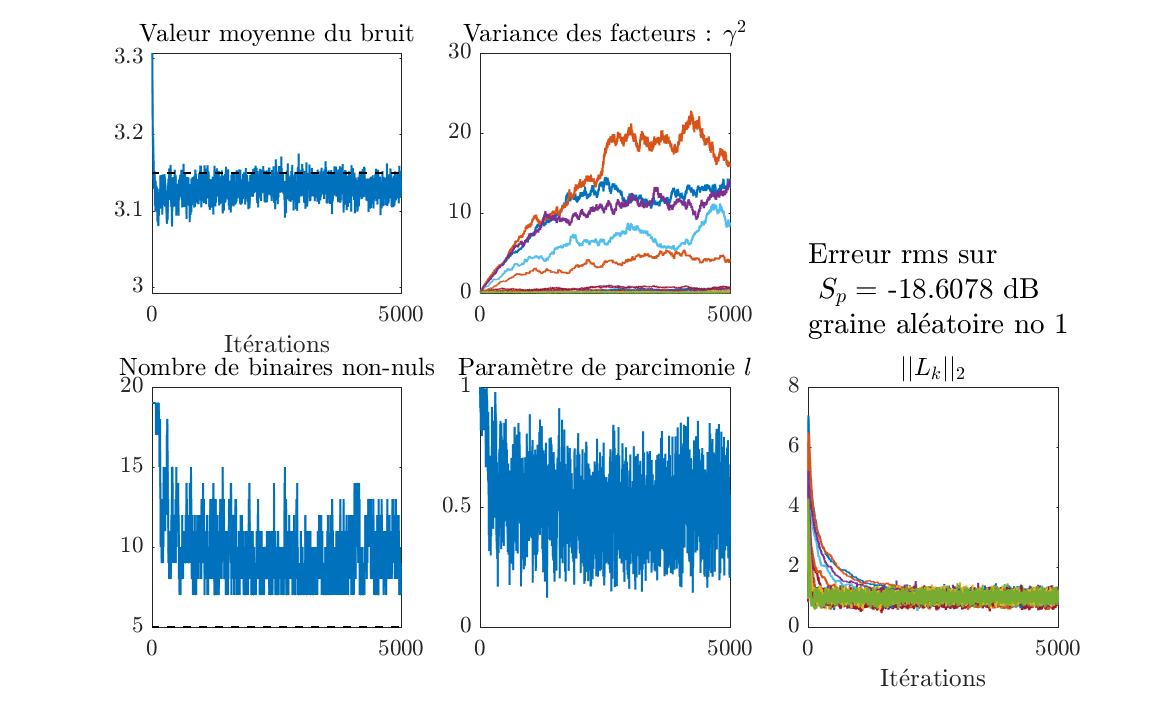
\includegraphics[width=\textwidth]{ToyCase/margon.png}
	\caption{SNR = 0 dB -- Modèle 2 AVEC marginalisation}
\end{figure}
\begin{figure}[H]
	\centering
	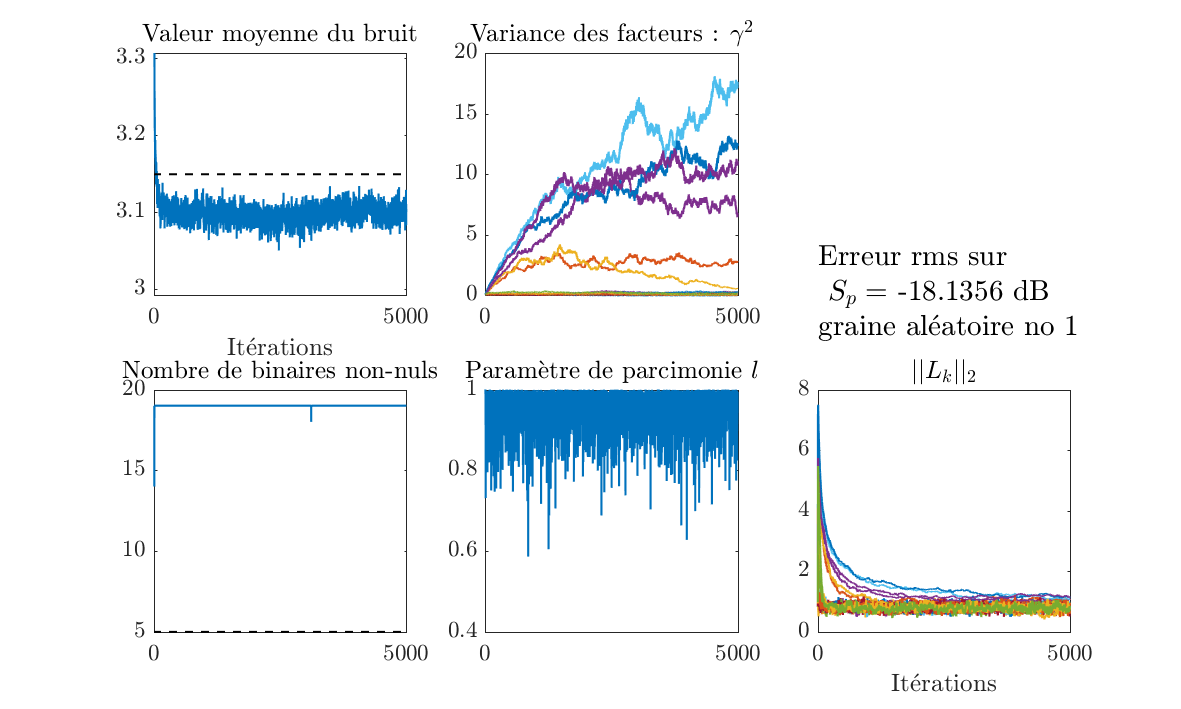
\includegraphics[width=\textwidth]{ToyCase/margoff.png}
	\caption{SNR = 0 dB -- Modèle 2 SANS marginalisation}
\end{figure}
\begin{figure}[H]
	\centering
	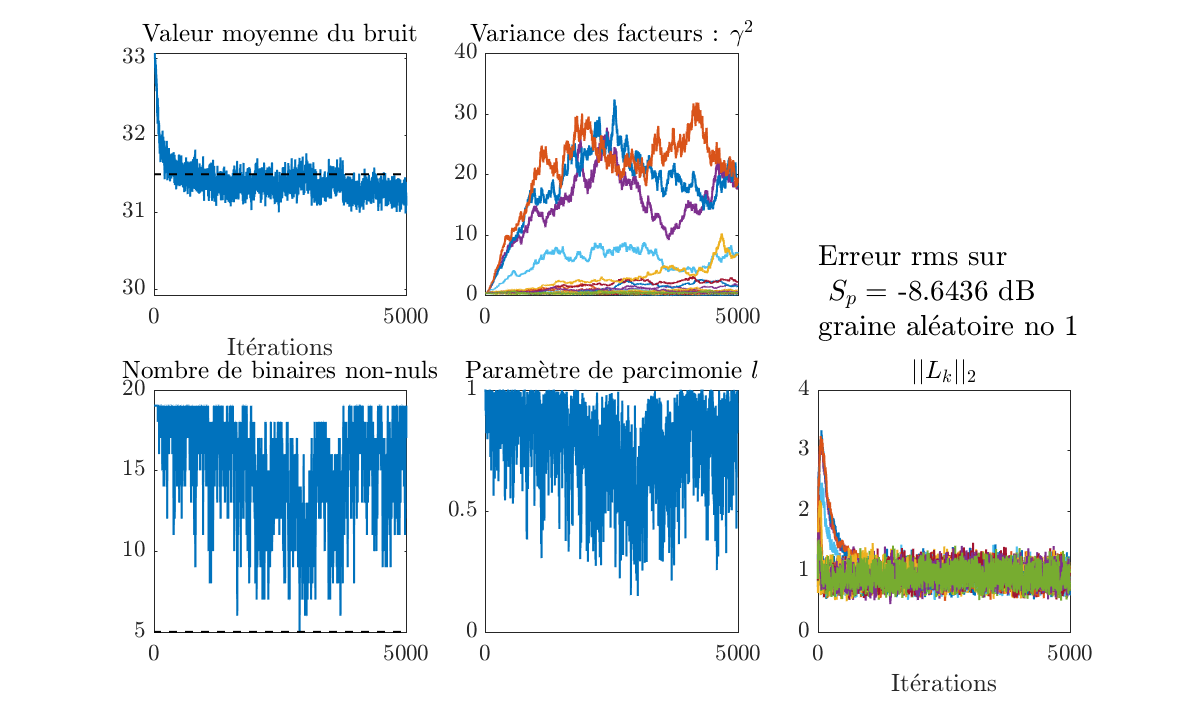
\includegraphics[width=\textwidth]{ToyCase/margon_snrm10db.png}
	\caption{SNR = -10 dB -- Modèle 2 AVEC marginalisation}
\end{figure}
\begin{figure}[H]
	\centering
	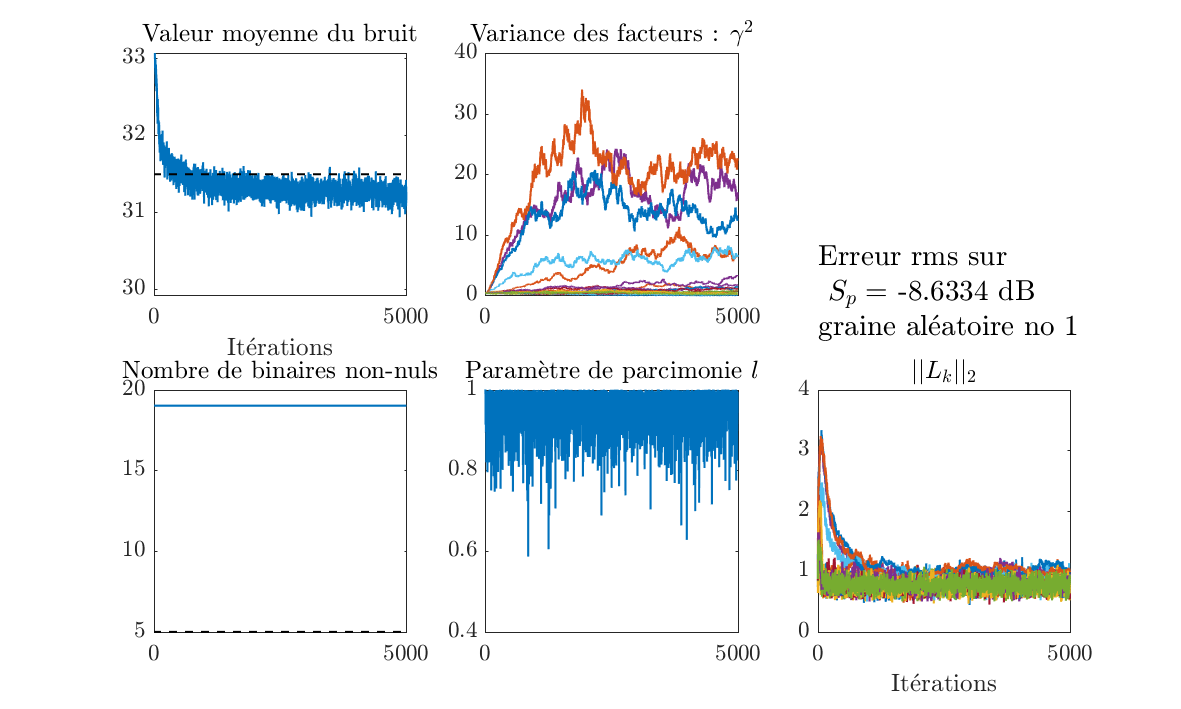
\includegraphics[width=\textwidth]{ToyCase/margoff_snrm10db.png}
	\caption{SNR = -10 dB -- Modèle 2 SANS marginalisation}
\end{figure}

\subsection{Effet de l'échantillonnage d'un facteur d'échelle}
\begin{figure}[H]
	\centering
	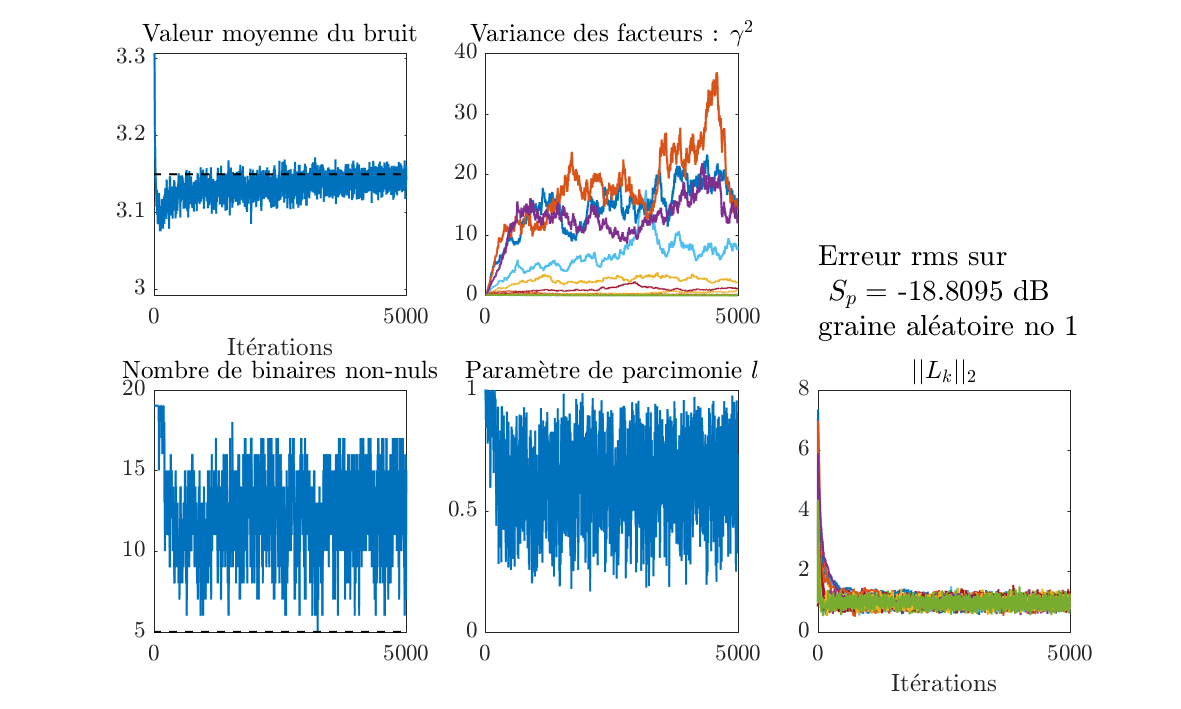
\includegraphics[width=\textwidth]{ToyCase/scalingon.png}\\
	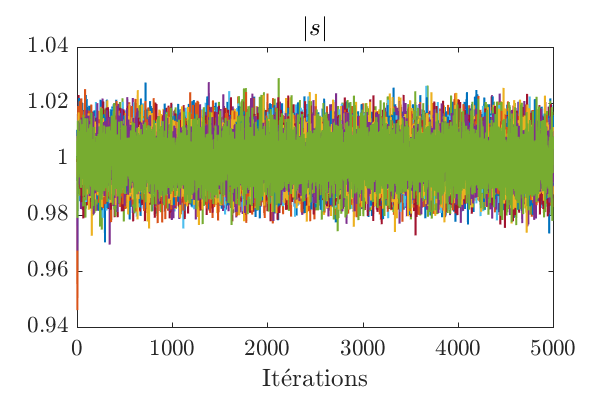
\includegraphics[width=0.4\textwidth]{ToyCase/s.png}
	\caption{SNR = 0 dB -- Modèle 2, avec marginalisation, AVEC échantillonnage d'un facteur d'échelle $s$.}
\end{figure}
\begin{figure}[H]
	\centering
	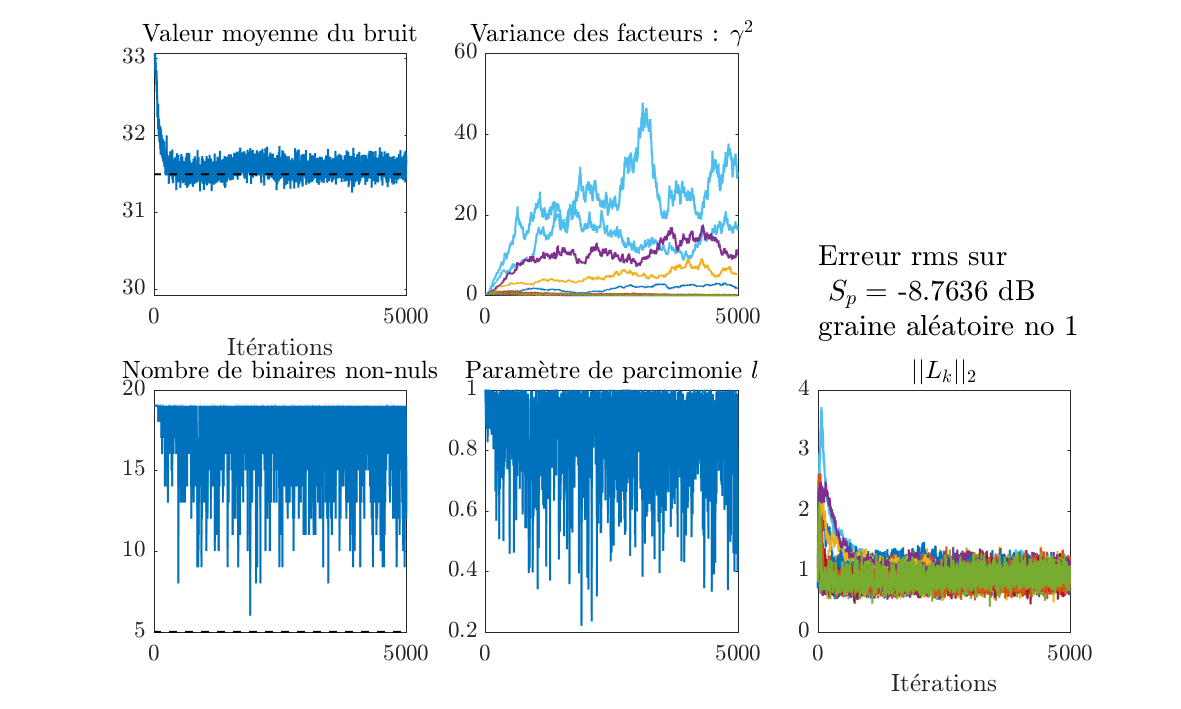
\includegraphics[width=\textwidth]{ToyCase/scalingon_snrm10db.png}\\
	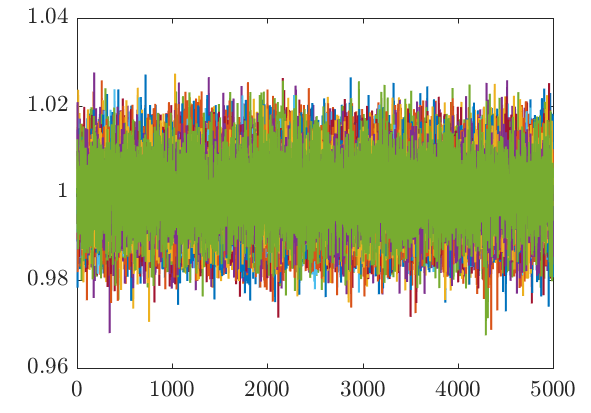
\includegraphics[width=0.4\textwidth]{ToyCase/s_snrm10db.png}
	\caption{SNR = -10 dB -- Modèle 2, avec marginalisation, AVEC échantillonnage d'un facteur d'échelle $s$.}
\end{figure}

\subsection{Modèle 2 : binaires fixés à 1}
\begin{figure}[H]
	\centering
	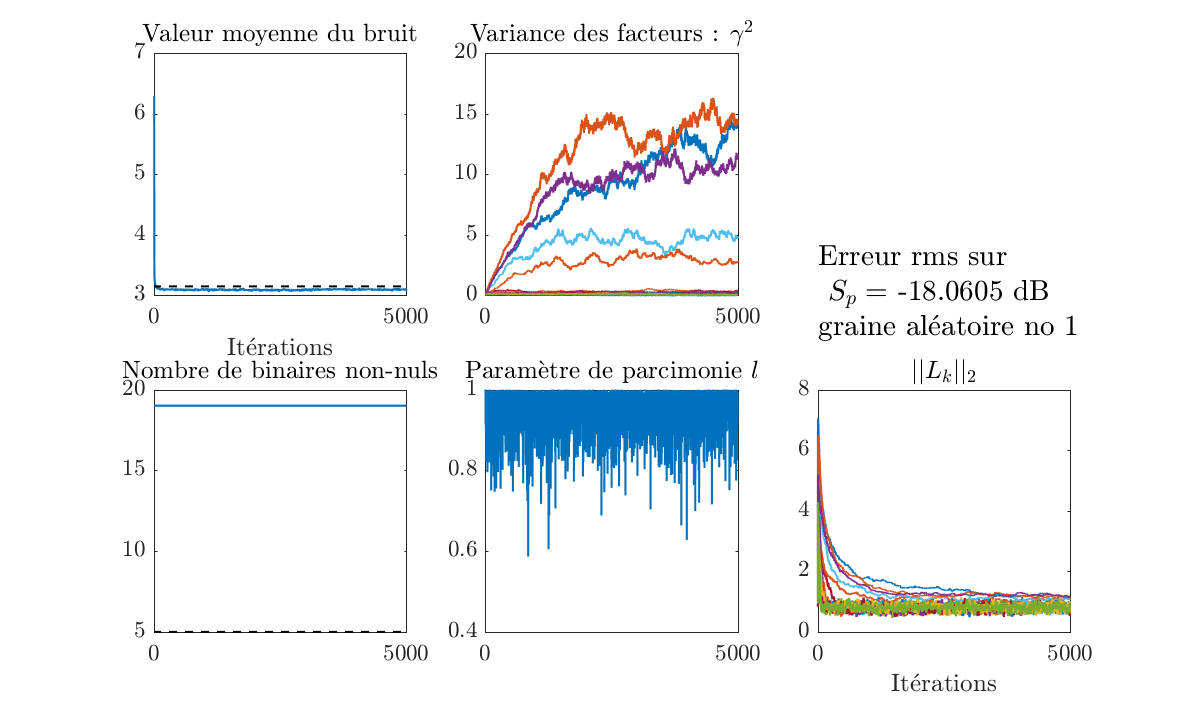
\includegraphics[width=\textwidth]{ToyCase/qfixe1.png}
	\caption{SNR = 0 dB -- Modèle 2, avec marginalisation, $\bm{q}=1$ (sans scaling).}
\end{figure}

\subsection{Modèle 2 : prior informatif sur $l$}
\begin{figure}[H]
	\centering
	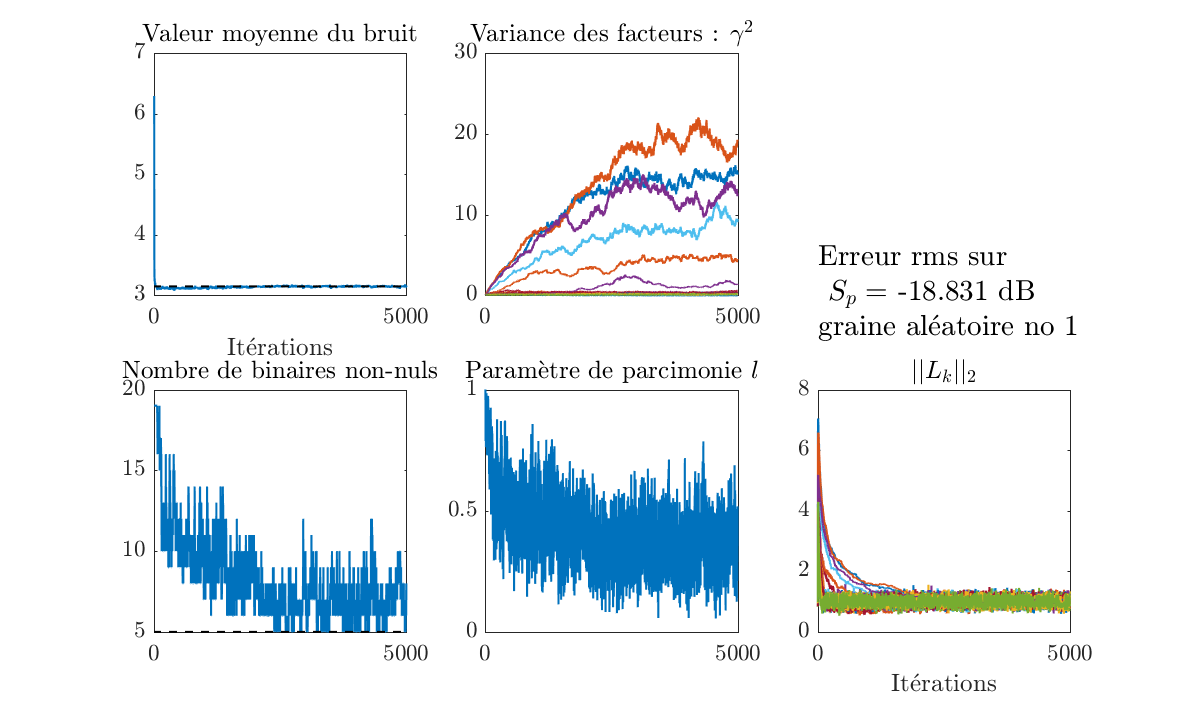
\includegraphics[width=\textwidth]{ToyCase/lsparse.png}\\
	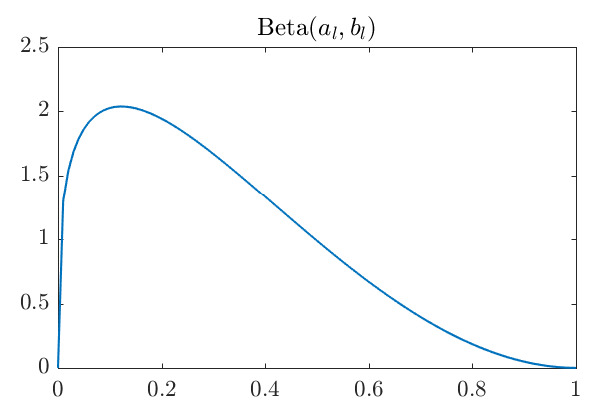
\includegraphics[width=0.4\textwidth]{ToyCase/priorl.png}
	\caption{SNR = 0 dB -- Modèle 2, avec marginalisation, le prior sur le paramètre de parcimonie $l$ n'est pas uniforme (sans scaling).}
\end{figure}
\begin{figure}[H]
	\centering
	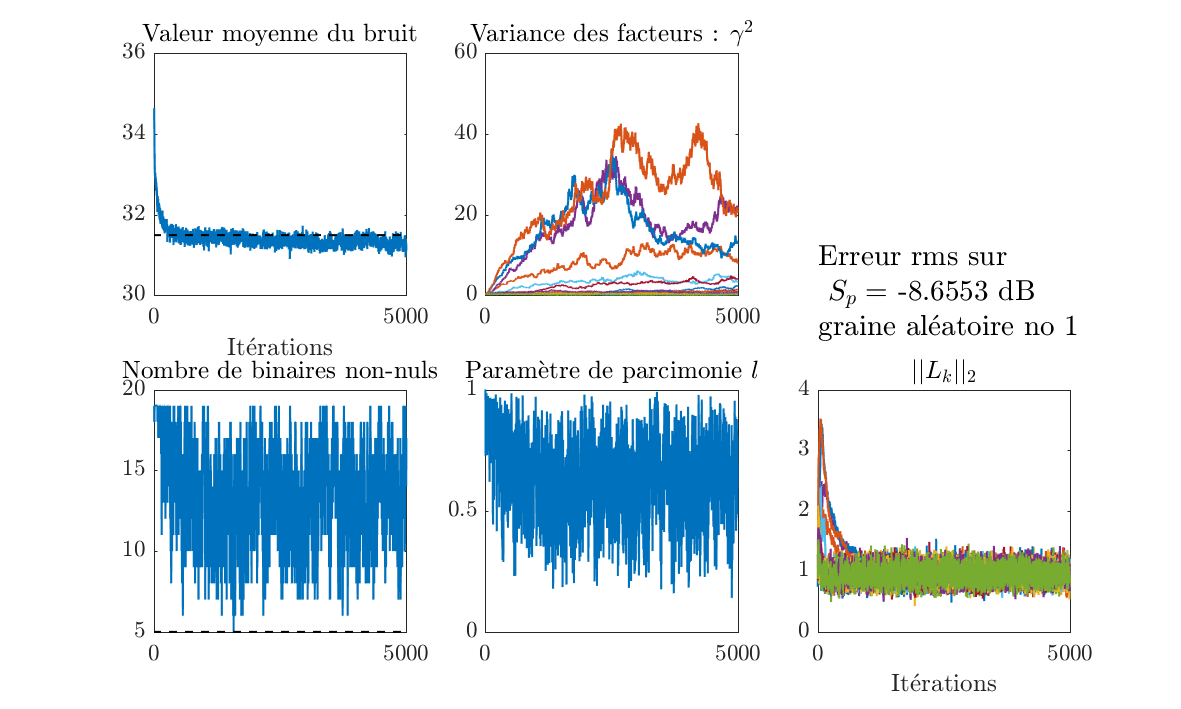
\includegraphics[width=\textwidth]{ToyCase/lsparse_snrm10db.png}
	\caption{SNR = -10 dB -- Modèle 2, avec marginalisation, le prior sur le paramètre de parcimonie $l$ n'est pas uniforme (sans scaling).}
\end{figure}

\newpage
\subsection{Comparaison avec le modèle 1}
\paragraph{$\bm{\gamma}^2 = \gamma^2\bm{I}_K$}
\begin{figure}[H]
	\centering
	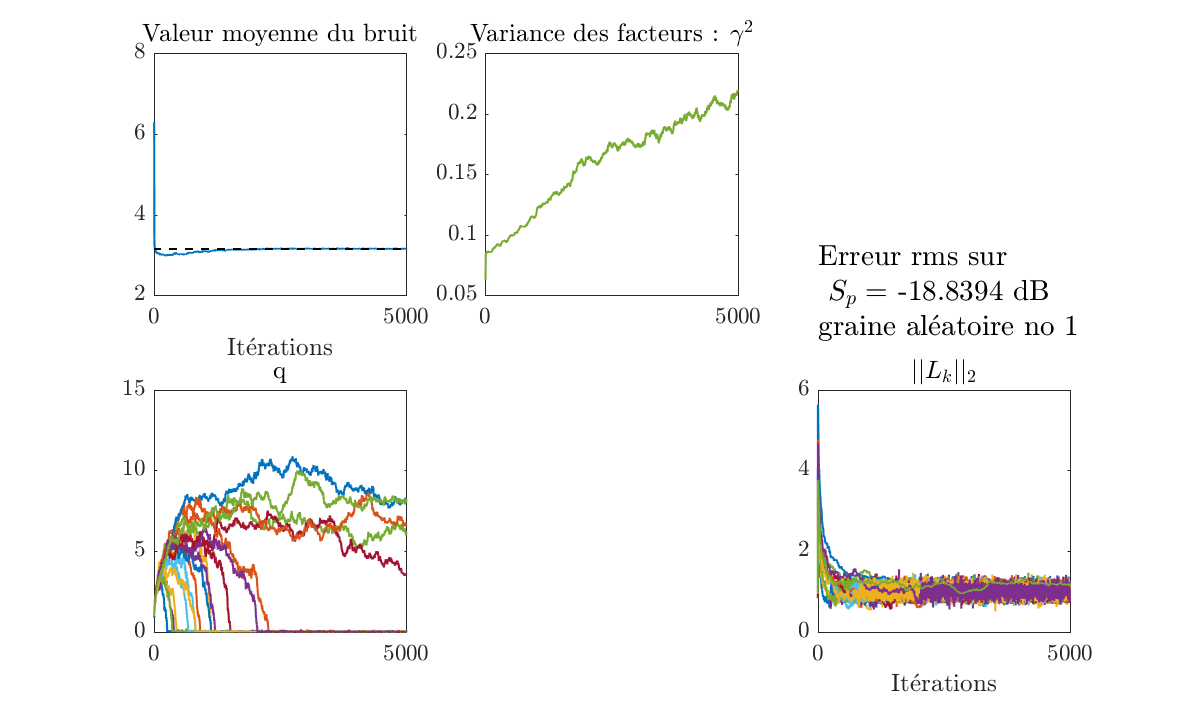
\includegraphics[width=\textwidth]{ToyCase/modele1.png}	
	\caption{SNR = 0 dB  -- Modèle 1, avec $\bm{\gamma}^2 = \gamma^2\bm{I}_K$ .}
\end{figure}
\begin{figure}[H]
	\centering
	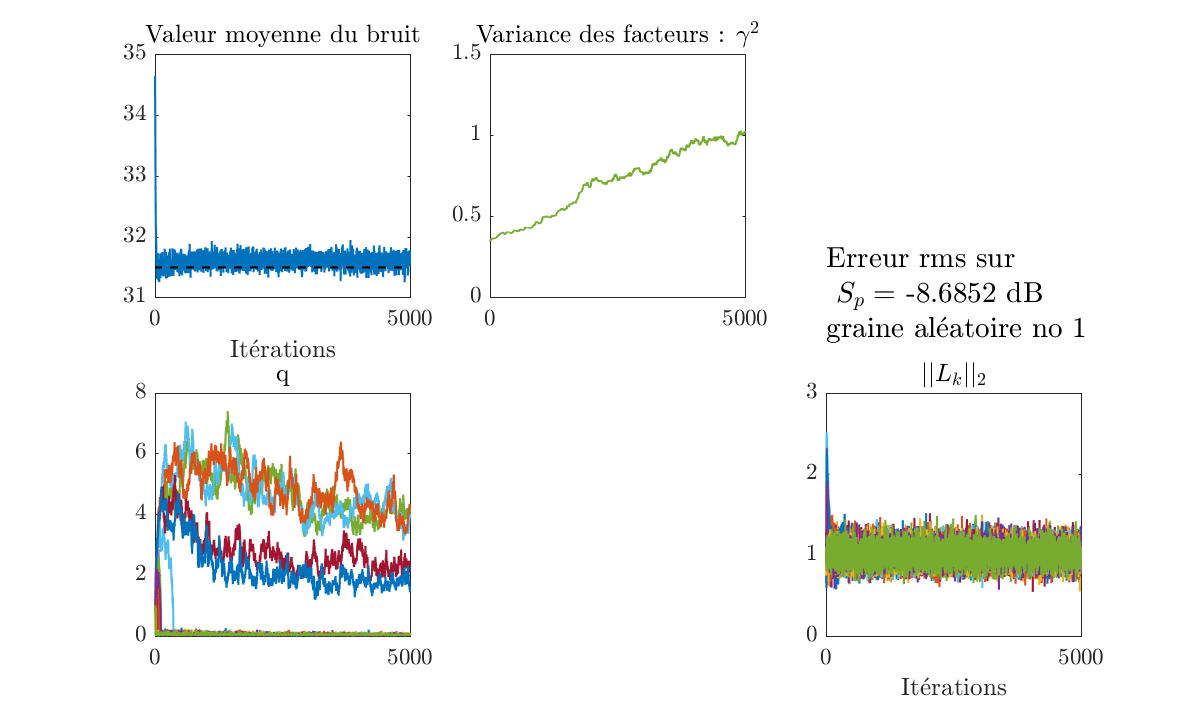
\includegraphics[width=\textwidth]{ToyCase/modele1_snrm10db.png}	
	\caption{SNR =-1 0 dB  -- Modèle 1, avec $\bm{\gamma}^2 = \gamma^2\bm{I}_K$ .}
\end{figure}

\paragraph{$\bm{\gamma}^2 = \diag{\bm{\gamma^2 }}$}
\begin{figure}[H]
	\centering
	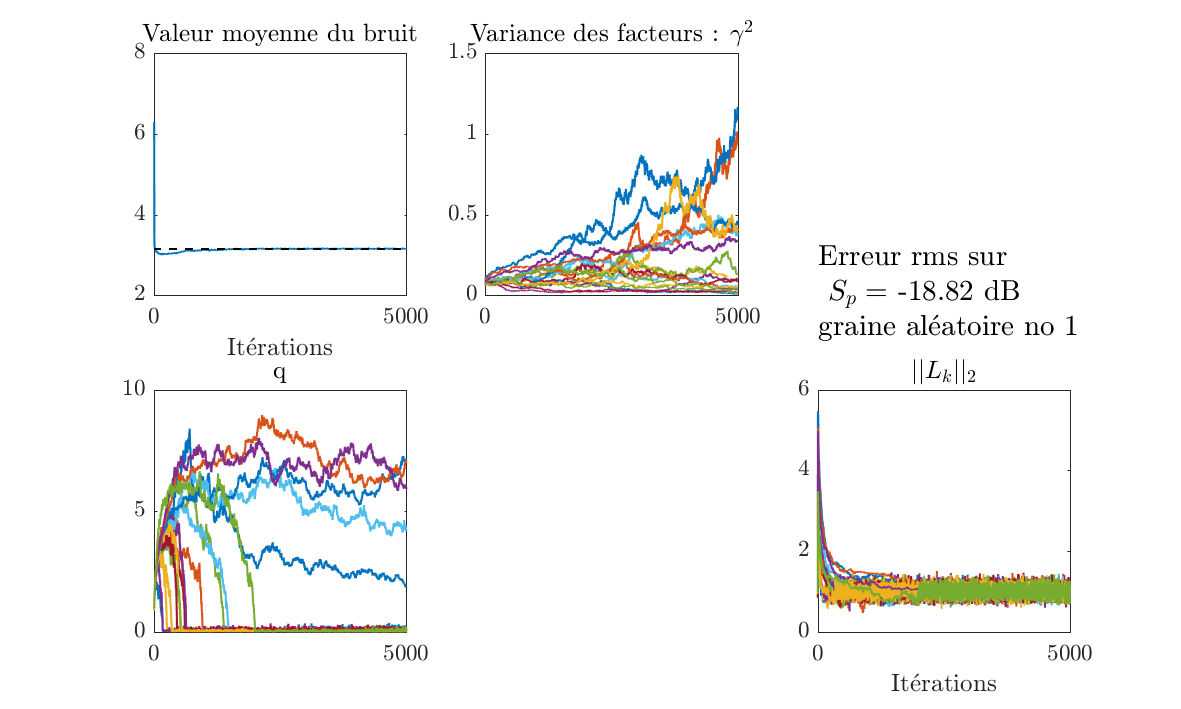
\includegraphics[width=\textwidth]{ToyCase/modele1_diffgamma2.png}	
	\caption{SNR = 0 dB  -- Modèle 1, avec $\bm{\gamma}^2  = \diag{\bm{\gamma^2 }}$ .}
\end{figure}
\begin{figure}[H]
	\centering
	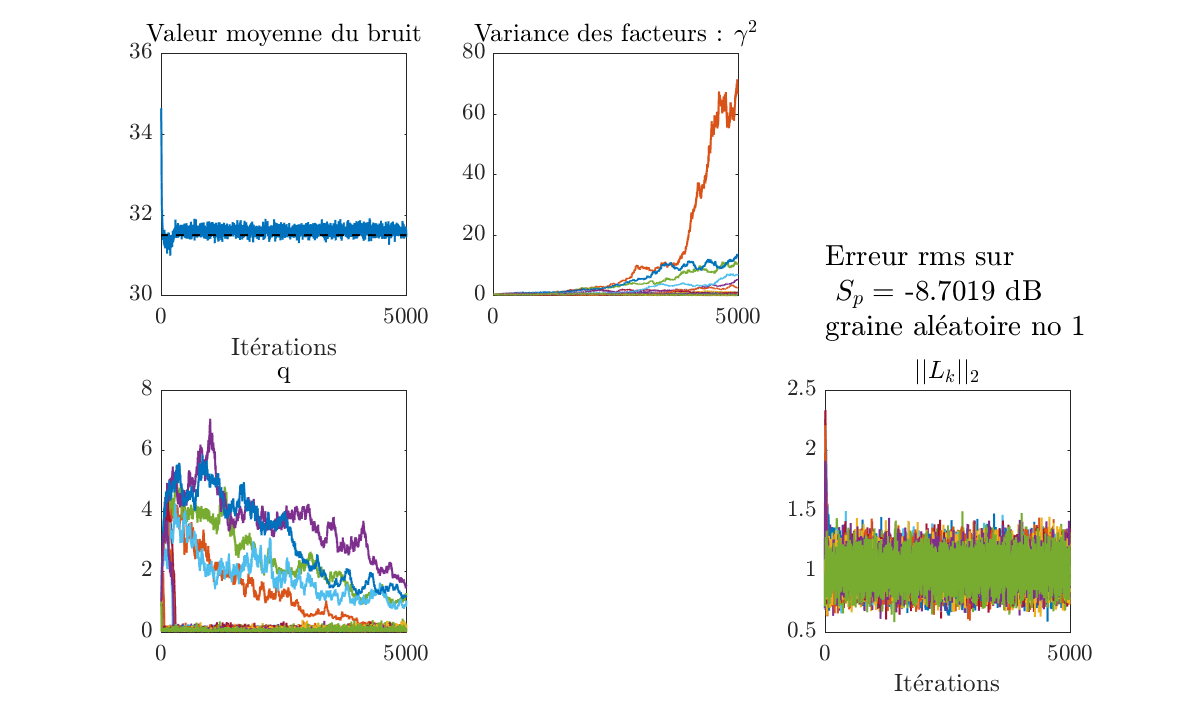
\includegraphics[width=\textwidth]{ToyCase/modele1_diffgamma2_snrm10db.png}	
	\caption{SNR = -10 dB  -- Modèle 1, avec $\bm{\gamma}^2  = \diag{\bm{\gamma^2 }}$ .}
\end{figure}

\todo[inline]{Le plus important : modèle 2 très sensible au choix de  a.alpha (ex : SVD ne marche pas bien. a.alpha=1 semble plus robuste. a.alpha=2 ne marche pas.\\
}


%\subsection{Sans marginalisation}
%
%\begin{figure}[H]
%\centering
%	\includegraphics[width = 0.32\linewidth]{./bern_nomarg_Sp_SNR0.png}
%	 \includegraphics[width = 0.32\linewidth]{./bern_nomarg_bruit_SNR0.png}
%	\includegraphics[width = 0.32\linewidth]{./bern_nomarg_gamma2_SNR0.png}\\
%	\includegraphics[width = 0.32\linewidth]{./bern_nomarg_q_SNR0.png}
%	\includegraphics[width = 0.32\linewidth]{./bern_nomarg_l_SNR0.png}
%	\caption{SNR = 0dB}
%\end{figure}
%\begin{figure}[H]
%\centering
%	\includegraphics[width = 0.32\linewidth]{./bern_nomarg_Sp_SNRm10.png}
%	 \includegraphics[width = 0.32\linewidth]{./bern_nomarg_bruit_SNRm10.png}
%	\includegraphics[width = 0.32\linewidth]{./bern_nomarg_gamma2_SNRm10.png}\\
%	\includegraphics[width = 0.32\linewidth]{./bern_nomarg_q_SNRm10.png}
%	\includegraphics[width = 0.32\linewidth]{./bern_nomarg_l_SNRm10.png}
%	\caption{SNR = -10dB}
%\end{figure}
%
%\newpage
%\subsection{Avec marginalisation}
%\begin{figure}[H]
%\centering
%	\includegraphics[width = 0.32\linewidth]{./bern_marg_Sp_SNR0.png}
%	 \includegraphics[width = 0.32\linewidth]{./bern_marg_bruit_SNR0.png}
%	\includegraphics[width = 0.32\linewidth]{./bern_marg_gamma2_SNR0.png}\\
%	\includegraphics[width = 0.32\linewidth]{./bern_marg_q_SNR0.png}
%	\includegraphics[width = 0.32\linewidth]{./bern_marg_l_SNR0.png}
%	\caption{SNR = 0dB}
%\end{figure}
%\begin{figure}[H]
%\centering
%	\includegraphics[width = 0.32\linewidth]{./bern_marg_Sp_SNRm10.png}
%	 \includegraphics[width = 0.32\linewidth]{./bern_marg_bruit_SNRm10.png}
%	\includegraphics[width = 0.32\linewidth]{./bern_marg_gamma2_SNRm10.png}\\
%	\includegraphics[width = 0.32\linewidth]{./bern_marg_q_SNRm10.png}
%	\includegraphics[width = 0.32\linewidth]{./bern_marg_l_SNRm10.png}
%	\caption{SNR = -10dB}
%\end{figure}
%
%\newpage
%\subsection{Comparaison avec l'ancienne version}
%\begin{figure}[H]
%\centering
%	\includegraphics[width = 0.32\linewidth]{./exp_Sp_SNR0.png}
%	 \includegraphics[width = 0.32\linewidth]{./exp_bruit_SNR0.png}
%	\includegraphics[width = 0.32\linewidth]{./exp_gamma2_SNR0.png}\\
%	\includegraphics[width = 0.32\linewidth]{./exp_q_SNR0.png}
%	\caption{SNR = 0dB}
%\end{figure}
%\begin{figure}[H]
%\centering
%	\includegraphics[width = 0.32\linewidth]{./exp_Sp_SNRm10.png}
%	 \includegraphics[width = 0.32\linewidth]{./exp_bruit_SNRm10.png}
%	\includegraphics[width = 0.32\linewidth]{./exp_gamma2_SNRm10.png}\\
%	\includegraphics[width = 0.32\linewidth]{./exp_q_SNRm10.png}
%	\caption{SNR = -10dB}
%\end{figure}
%%
%
%
%\textbf{Remarques : }
%\begin{itemize}
%        \item Les résultats issus du modèle 2 changent beaucoup en fonction de l'initialisation, mais comme la convergence est rapide (surtout quand le SNR n'est pas trop bas), il serait possible de lancer simultanément plusieurs chaîne avec différentes initialisations, plus courtes.
%        \item Il serait intéressant de comparer les résultats dans le cas où le nombre de fonction de bases est grand (hypothèse de parcimonie non respectée)
%\end{itemize}


\section{Problème d'échelle}
\subsection[]{Pour le couple $\bm{c},\bm{L}$}

\cite{veit2008reechantillonnage} propose un moyen de gérer l’ambiguïté d'échelle entre les paramètres $\bm{c}$ et $\bm{L}$. D'après cet article, lever cette ambiguïté permettrait une exploration de la loi cible plus efficace, avec une meilleure mélangeance, en réduisant le temps de chauffe et la corrélation de ces paramètres. 
De manière générale, cette ambiguïté se retrouve pour tout problème de la forme : 
\begin{equation*}
	    z=h \star x + b
\end{equation*}
où $\star$ est un opérateur bilinéaire quelconque, un produit matriciel dans notre cas. En effet, on a alors, pour tout couple $(x,h)$ et $s \neq 0$ :
\begin{equation*}
	    (sx) \star \left(\frac{h}{s} \right) = x \star h
\end{equation*}
\cite{veit2008reechantillonnage} propose donc d'échantillonner le paramètre de changement d'échelle sans modifier la loi cible. Dans notre modèle, il faut un facteur d'échelle $s_k$ par facteur :
\begin{equation*}
	    \bm{y} =  \bm{Lqc}+ \bm{n} = (\bm{\tilde{L}S}^{-1}) \bm{q}(\bm{S\tilde{c}}) + \bm{n} \quad \text{avec} \quad \bm{S} = \operatorname{diag}(s_1, \dots , s_k, \dots , s_K).
\end{equation*}
On peut montrer par un changement de variable 

\begin{align*}
	\bm{L}_k = \frac{\tilde{\bm{L}}_k}{s_k} \quad \text{et} \quad \bm{c_k} = \tilde{\bm{c}}_k s_k
\end{align*}
que l'échantillonnage de $s_k$ se fait selon la loi 
\begin{equation}
        [s_k|\infty_{-s_k}] \propto |s_k|^{2(I_s - M -1)} [ \bm{c}_k,\bm{L}_k| s_k] 
\end{equation}
Sous l'hypothèse d'indépendance de $\bm{c}_k$ et $\bm{L}_k$, 
\begin{equation}
        [s_k|\infty_{-s_k}] \propto |s_k|^{2(I_s - M -1)} \prod_i [ \bm{c}_{ki}] \prod_m[\bm{L}_{mk}] .
\end{equation}
avec $|s_k|^2 = ss^*$.

En posant $r_k=|s_k|^2$, on en déduit que 
\begin{align*}
	[r_k|\infty] & \propto r_k^{I_s -M -\frac{1}{2} -1} \e^{-r_k\sum_i \bm{\tilde{c}}_{ki}^H \gamma_k^{-2}\bm{\tilde{c}}_{ki}} \quad
	 \e^{-r_k^{-1}\sum_m \bm{\tilde{L}}_{mk}^H K \bm{\tilde{L}}_{mk}}\\
	 & \propto r_k^{I_s -M -\frac{1}{2} -1}  \e^{-r_k  \gamma_k^{-2} \bm{\tilde{S}}_{{cc}_{kk}}} \quad
	 	\e^{-r_k^{-1}K \sum_m \bm{\tilde{L}}_{mk}^H \bm{\tilde{L}}_{mk}}
			%& \propto r^{\frac{K-MK-1}{2}} \e^{-r \tr{ \bm{\gamma}^{-2} \bm{S}_{cc}} - r^{-1} K \bm{\lambda}^H \bm{\lambda}}
\end{align*}

$r$ suit donc une loi Gaussienne Inverse Généralisée (GIG)  de la forme : 
\begin{equation*}
	    f_{GIG}(r) = \left(\frac{a_r}{b_r}\right)^{\frac{p_r}{2}}  \frac{r^{p_r-1}}{2 \operatorname{Y}_{p_r}\!\left( \sqrt{a_rb_r}\right)} \e^{-\frac{1}{2} ( a_r r + b_r r^{-1} )} \quad, r>0
\end{equation*}
$ \operatorname{Y}_{p_r} (\cdot)$ est la fonction de Bessel de seconde espèce.

Par identification, les paramètres sont : 
\begin{align*}
	a_{r_k} & = 2 \gamma_k^{-2}\bm{\tilde{S}}_{{cc}_{kk}}\\
	b_{r_k} &= 2K \sum_m \bm{\tilde{L}}_{mk}^H \bm{\tilde{L}}_{mk}\\
	p_r &= I_s- M - \frac{1}{2}
\end{align*}
Après tirage de $r_k$, on calcule $s_k=\sqrt{r_k} \e^{j\phi}$ avec $\phi \sim \mathcal{U}([0;2\pi[)$.

Dans le cas où $M\approx K \ll I_s$, les paramètres sont de l'ordre de grandeur suivant :
\begin{align*}
	a_{r_k} &\approx 2 I_s\\
	b_{r_k} &\approx 2M\\
	p_r &\approx  I_s-M
\end{align*}
le mode de la GIG est alors :
\begin{align*}
	\mathrm{mode}_{GIG} & = \frac{(p_r -1) + \sqrt{(p_r-1)^2 + a_rb_r}}{a_r}\\
	& \approx \frac{I_s + \sqrt{I_s^2}}{2I_s} \approx 1
\end{align*}
et la variance est très faible.
Le paramètre d'échelle oscille donc légèrement autour de 1, ce qui ne modifie pas l'échelle du problème.\\


\subsection[]{Pour le couple $\beta^2, \bm{\sigma}^2$}
L’ambiguïté se pose également pour le couple $\beta^2, \bm{\sigma}^2$ dans le cas où on exploite P jeux de données (pour différents régime moteur par ex.).
On note $\bm{\beta}^2$ le vecteur contenant les $P$ valeurs réelles de $\beta^2_p$ et $\bm{\sigma}^2$ celui contenant les $M$ valeurs réelles $\sigma_m^2$.. Le facteur d'échelle s suit alors la loi suivante : 
\begin{align*}
	[s |\infty] &\propto |s|^{P-M-1} \prod_p [s \beta_p^2] \prod_m [s^{-1}\sigma_m^2]\\
	& \propto |s|^{P-M-1} \quad\e^{-\sum_p \beta_p^{-2} b_\beta s^{-1}} \e^{- \sum_m \sigma_m^{-2} b_\sigma s}\\
	& \propto \mathcal{GIG}(2 \sum_m \sigma^{-2}_m b_\sigma, 2 \sum_p \beta^{-2}_p b_\beta, P-M)
\end{align*}
s doit être réel et son signe est tiré dans une loi uniforme $\mathcal{U}([0;1])$.



\newpage
\appendix
%\@seccntformat#1{Appendix~\csname the#1\endcsname:\quad}
\titleformat{\section}[block]{\bfseries\centering}{Annexe \thesection.}{1em}{}
\section{Détail du calcul de la postérieure marginalisée \label{demo_marg}}

La marginalisation revient à projeter la loi conjointe $[\bm{y}_i,\bm{c}_i]$sur $\bm{c}_i$ :
\begin{align*}
        [\bm{y}_i | \infty_{-\bm{c}}] &= \int [\bm{y}_i,\bm{c}_i]  \operatorname{d}\!\bm{c}_i\\
        		&= \int [\bm{y}_i | \bm{c}_i ][\bm{c}_i] \operatorname{d}\!\bm{c}_i
\end{align*}
Or,
\begin{align*}
	 [\bm{y}_i | \bm{c}_i ][\bm{c}_i] &= \e^{(\bm{y}_i - \bm{Lqc}_i)^H \bm{\sigma_n^{-2}}(\bm{y}_i - \bm{Lqc}_i)} \e^{\bm{c}^h \bm{\gamma}^{-2}\bm{c}_i}\\
	 		&= \e^{-\bm{y}_i^H\bm{\sigma}_n^{-2}\bm{y}_i}
	 		\	\e\underbrace{^{(\bm{Lqc}_i)^H\bm{\sigma}_n^{-2}\bm{y}_i}}_{ \bm{c}_i\bm{\Omega}_{\bm{c}_i}^{-1} \bm{\mu}_i}
	 		\	\e\underbrace{^{\bm{y}_i^H\bm{\sigma}_n^{-2}\bm{Lqc}_i}}_{\bm{\mu}_i^H \bm{\Omega}_{\bm{c}_i}^{-1}\bm{c}_i}
	 		\	\e\underbrace{^{-(\bm{Lqc}_i)^H \bm{\sigma}_n^{-2}\bm{Lqc}_i}}_{-\bm{c}_i^H \bm{\Omega}_{\bm{c}_i}^{-1}\bm{c}_i}\\
	 		&= \bm{C}_1 \e^{-(\bm{c}_i-\bm{\mu}_i)^H \bm{\Omega}_{\bm{c}_i}(\bm{c}_i-\bm{\mu}_i) }
\end{align*}
avec $\bm{\mu}_i$ et $\bm{\Omega}_{\bm{c}_i}$ sont donnés dans l'encart~\eqref{eq:c}. Donc,
\begin{equation*}
	      [\bm{y}_i | \infty_{-\bm{c}}]  = \int [\bm{y}_i | \bm{c}_i ][\bm{c}_i] \operatorname{d} \bm{c}_i = \bm{C}_1 \underbrace{ \int \mathcal{N}_c(\bm{\mu}_i, \bm{\Omega}_{\bm{c}_i})\operatorname{d}\!\bm{c}_i }_{=1}= \bm{C}_1
\end{equation*}



Par identification, 
\begin{align*}
	    & \bm{C}_1\ \e^{-\bm{\mu}_i^H   \bm{\Omega}_{\bm{c}_i \bm{\mu}_i   }} = \e^{-\bm{y}_i^H \bm{\sigma}_n^{-2} \bm{y}_i}\\
	    \Leftrightarrow \quad & \bm{C}_1 = \e^{-\bm{y}_i^H\bm{\sigma}_n^{-2}\bm{y}_i} \ \e\underbrace{^{\bm{y}_i^H \bm{\sigma}_n^{-2} \bm{Lq \Omega}_{\bm{c}_i} \bm{q}^H \bm{L}^H  \bm{\sigma}_n^{-2}\bm{y}_i}}_{\bm{A}}\\
	    & \bm{C}_1 = \e^{-\bm{y}_i ^H \bm{B}^{-1} \bm{y}_i}
\end{align*}
avec 
\begin{equation*}
	    \bm{A} = \frac{\bm{\sigma}_n^{-2}}{1 + \underbrace{\bm{L}^{H^{-1}} \bm{q}^{H^{-1}} \bm{\gamma}^{-2} \bm{q}^{-1}\bm{L}^{-1} }_{\bm{A}_2^{-1}} \bm{\sigma}_n^{2}}
\end{equation*}
et 
\begin{align*}
	    \bm{B}^{-1} & = -\bm{A} + \bm{\sigma}_n^{-2}  = \frac{\bm{- \sigma}_n^{-2} + \bm{\sigma}_n^{-2} \left( 1+ \bm{A}_2^{-1} \bm{\sigma}_2^2\right)}{1+  \bm{A}_2^{-1}\bm{\sigma}_n^{2}}\\
	    & = \frac{1}{\bm{A}_2 + \bm{\sigma}_n^2}
\end{align*}
Finalement, 
\begin{equation*}
	      [\bm{y}_i | \infty_{-\bm{c}}]  = \bm{C}_1 = \mathcal{N}_c(\bm{0}, \bm{B}) \quad \text{où} \quad \bm{B} = \bm{Lq \gamma}^2 \bm{q}^H \bm{L}^H +\bm{\sigma}_n^2 .
\end{equation*}






 



\bibliographystyle{plainnat}
\bibliography{biblio}



\end{document}
